%!TEX root = ../main.tex
\chapter{Grundlagen}
\label{cha:Grundlagen}
Das folgende Kapitel beschäftigt sich mit Grundlagen, derer Kenntnis in der weiteren Arbeit vorausgesetzt wird. Im Vordergrund stehen hierbei die Erläuterung der agilen Arbeitsweise und Scrum, insbesondere die individuellen Anpassungen bei kernpunkt, sowie ein kurzer Überblick über den bisherigen Prototypen und den menschzentrierten Entwicklungsprozess.

\section{Agilität und Scrum}
\label{sec:agilitaet_scrum}
Im Jahr 2001 wurde das agile Manifest von der \textit{The Agile Alliance}, einem Verbund von 17 Softwareentwicklern und Projektleitern aus dem IT-Umfeld, entwickelt und unterzeichnet \cite{agilemanifestosignatories, agilemanifestohistory}. 
\begin{quote}
''Agile Softwareentwicklung bezeichnet Ansätze im Softwareentwicklungsprozess, die die Transparenz und Flexibilität erhöhen und zu einem schnelleren Einsatz der entwickelten Systeme führen sollen, um so Risiken im Entwicklungsprozess zu minimieren. Die Kernidee besteht darin, Teilprozesse möglichst einfach und somit beweglich (=agil) zu halten.''\cite{definitionagil}.
\end{quote}
Das agile Manifest sollte eine Alternative zu den bisherigen schwergewichtigen und unflexiblen Entwicklungsprozessen, wie beispielsweise dem Wasserfallmodell, aufzeigen, welches auf kurzfristige Ereignisse schnell reagieren und sich so besser individualisieren und anpassen lässt \cite{agilemanifestohistory}. \\ \\
Auf Grundlage dieses Manifestes entstanden verschiedene Frameworks und Arbeitsweisen, darunter Scrum. Das Rahmenwerk \textit{Scrum} wurde von Ken Schwaber und Jeff Sutherland, zwei Mitgliedern der Agile Alliance, bereits in den frühen 1990er-Jahren erfunden und entwickelt. Es existiert nach eigener Aussage, damit  ''Menschen komplexe adaptive Aufgabenstellungen angehen können'', um ''[...] produktiv und kreativ Produkte mit höchstmöglichem Wert auszuliefern.'' \cite{scrumguide}.
\\ \\
Im Mittelpunkt von Scrum stehen selbstorganisierte Teams. Ein solches Team besteht aus Teammitgliedern, einem \textit{Product Owner} und einem \textit{Scrum Master}. Die Teammitglieder, im Gesamten auch Entwicklungsteam genannt, sind der Kern und dienen der Herstellung des Produktes, in diesem Fall der Entwicklung von Software. Wichtig ist hierbei, dass das Team über alle Fähigkeiten verfügt, um seine Aufgaben lösen zu können. Dementsprechend arbeitet es interdisziplinär in verschiedenen Gewerken. Laut Scrum Guide sollte ein Team aus drei bis neun Mitgliedern bestehen. Die Verantwortlichkeit liegt stets beim gesamten Team und nicht bei einzelnen Personen, auch wenn diese bestimmte Tätigkeitsfelder und Fähigkeiten besitzen.
\\ \\
Der Scrum Master dient zur Betreuung und Unterstützung des Scrum-Prozesses. Dazu leitet er die verschiedenen Termine und achtet auf Einhaltung der zeitlichen Rahmen. Eine weitere wichtige Rolle ist das Lehren von Scrum, sowohl im Team und im Unternehmen, als auch bei Stakeholdern, um ihnen den agilen Prozess im Team zu verdeutlichen und so die Qualität der Arbeit zu maximieren. Dabei agiert der Scrum Master als ''Servant Leader'' \cite{scrumguide}. Das bedeutet, dass er die Bedürfnisse des Teams identifiziert und sie möglichst befriedigt, ohne seine Führung zu vernachlässigen \cite{servantleadership}. 
\\ \\
Der Product Owner ist verantwortlich für den Wert der Arbeit der Teammitglieder und den wirtschaftlichen Erfolg. Außerdem ist er allein zuständig für das \textit{Product Backlog}. Das Product Backlog ist eine Auflistung aller Aufgaben, die nötig sind, um das Produkt herzustellen. Es ist flexibel, neue Aufgaben können hinzukommen, andere können entfernt werden, abhängig von den Anforderungen an das Produkt. Das Backlog wird vom Product Owner priorisiert, auch ist er zuständig für eine ausreichende Beschreibung der Aufgaben. Er steht im Dialog mit den Stakeholdern, um auf Anforderungsänderungen und Kundenwünsche reagieren zu können.
\\ \\
Die Aufgaben werden in sogenannten User Stories verfasst. Eine User Story ist ein Format in der Anforderungen in einer verständlichen, nicht technischen Sprache festgehalten werden \cite{userstoryformat}. Außerdem enthält sie Unteraufgaben und Akzeptanzkriterien, die erfüllt sein müssen, um eine Story als erledigt zu beschreiben. Die genaue Definition einer erledigten Story, auch \textit{Definition of Done} genannt und ''wird dazu verwendet festzustellen, wann die Arbeit an einem Produktinkrement fertig ist'' \cite{scrumguide}. Zur Komplexitätseinschätzung werden Stories vom Team mit \textit{Story Points} versehen. Story Points sind eine relative Einheit und unterscheiden sich in jedem Team. Mögliche sind alle Werte der Fibonacci-Folge bis 100, wobei ab 21 auf den vorherigen Zehner abgerundet wird \cite{storypoints}. Die Schätzung erfolgt im sogenannten \textit{Product Backlog refinement}, in welchem sich das Entwicklungsteam allein die Story Points festlegt, wobei der Product Owner aufs Team einwirken kann, indem ''er ihm beim Verständnis der Einträge hilft oder Kompromisse eingeht'' \cite{scrumguide}.
\\ \\
Der zeitliche Rahmen zur Bearbeitung von Stories wird durch den \textit{Sprint} festgelegt. Ein Sprint ist ein zeitlicher Rahmen, in welchem Aufgaben erledigt werden sollen, die ein Produktinkrement erzeugen, das zu Sprintende ausgeliefert werden kann. Ein Sprint darf eine länge von einem Monat nicht überschreiten und wird zu Beginn im sogenannten \textit{Planning} strukturiert und vorbereitet. So werden im Planning alle Stories bestimmt, die innerhalb des Sprints bearbeitet und fertiggestellt werden sollen. Diese Stories werden vom Product Backlog ins Sprint Backlog verschoben, müssen allerdings bereits geschätzt worden sein. Hat sich das Team auf einen Sprint geeinigt, wird dieser gestartet. Ab diesem Zeitpunkt arbeitet das Team an seinen Aufgaben, um das \textit{Sprint-Ziel} zu erreichen. Um dies zu erreichen, werden während des Sprints keine Änderungen vorgenommen, die dieses Ziel gefährden. 
\\ \\
Damit der aktuellen Fortschritt im Team transparent und sichtbar ist, findet täglich das \textit{Daily Scrum} statt. Hier erläutert jedes Teammitglied kurz, welche Story es am vorherigen Tag bearbeitet hat, welche es nun bearbeiten wird und ob es durch Probleme, auch \textit{Impediments} genannt, an der Fertigstellung von Aufgaben verhindert wird. Schwierigkeiten im Entwicklungsprozess und neue sich ergebende Anforderungen werden hier offen an den Product Owner kommuniziert. Das Daily Scrum (oder kurz: Daily) findet am Scrumboard statt, mehr dazu in Kapitel \ref{sec:digitale_analoge_boards}.
\\ \\ 
Wie bereits erwähnt soll dem Kunden zu Ende eines Sprints ein Produktinkrement ausgeliefert werden. In der \textit{Sprint Review} wird dieses Inkrement den Stakeholdern vorgestellt und so das Ergebnis des Sprints präsentiert. Hier sollen neue Anforderungen aufgenommen werden, die die Basis für weitere User Stories bilden. Auch die aufgetretenen Probleme werden vom Entwicklungsteam vorgestellt. Nach der Review findet zum Abschluss des Sprints die Retrospektive statt. Dieser interne Termin dient zum Rückblick auf den letzten Sprint angesichts der Vorgehensweise und zur Erarbeitung neuer Maßnahmen, die den nächsten Sprint und somit den agilen Arbeitsprozess verbessern sollen.

\section{Analoge und Digitale Scrumboards}
\label{sec:digitale_analoge_boards}
Ein fester Bestandteil des Scrum-Frameworks ist das \textit{Scrumboard}. Es ist eine Abbildung des Sprint Backlogs und dient der Visualisierung von Stories, derer Unteraufgaben und jeweiligen Status. So kann eine Story drei verschiedene Status annehmen. \textit{To Do} bedeutet, dass die Story sich bereits im Sprint befindet, ihre Bearbeitung jedoch noch nicht begonnen hat. Sobald die Bearbeitung beginnt, befindet sie sich \textit{In Work}. Ist sie fertiggestellt und entspricht der Definition of Done, ist ihr Status \textit{Done}. Diese Status werden auf dem Board meist durch drei Spalten dargestellt. 
\\ \\
\begin{figure}[!ht]
	\centering
		%[natürliche Breite in Pixeln, natürliche Höhe in Pixeln, Abhängigkeit von der Textbreite]
		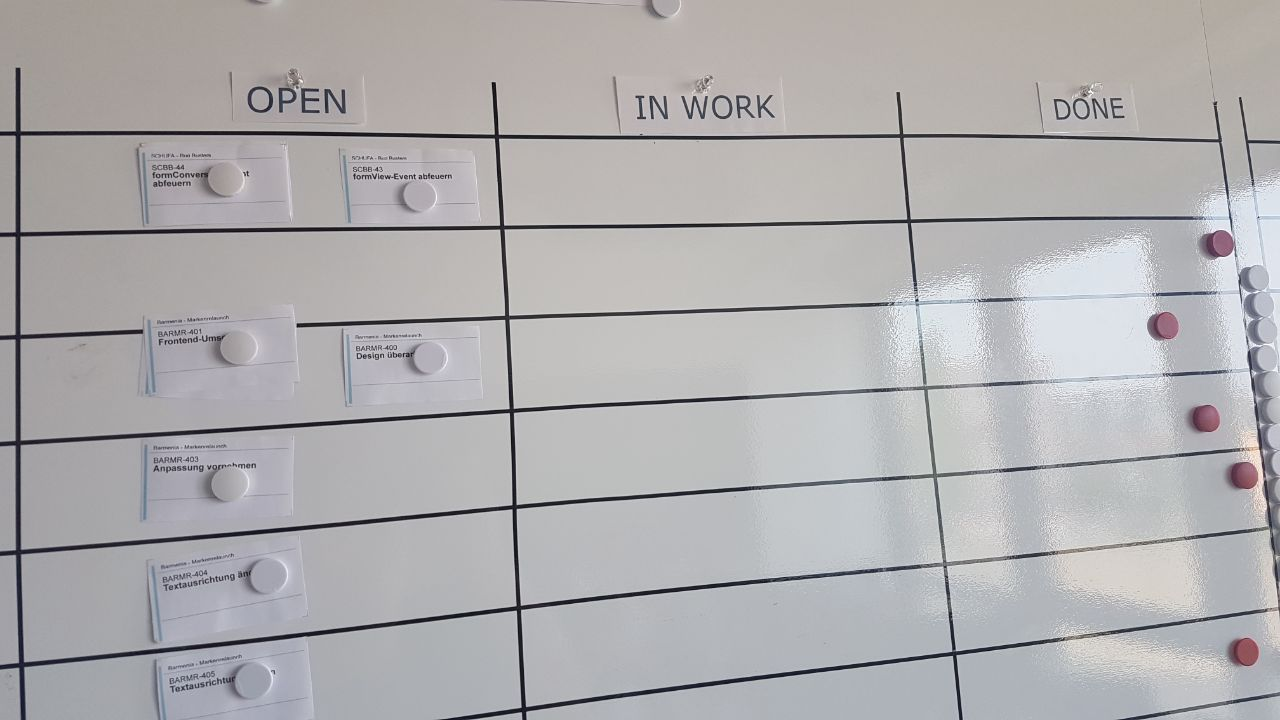
\includegraphics[width=0.75\textwidth]{images/physicalBoardNear.jpg}
	\caption{Bildunterschrift mit einer Quelle}
	\label{fig:box}
\end{figure}

HIER MUSS DIE EMPIRIE REIN

\section{Architektur und Prototyp zur Synchronisation von Boards}
\label{sec:architektur_prototyp_sync}

Architektur und Prototyp zur Synchronisation von Boards

\section{Menschzentrierter Entwicklungsprozess nach ISO 9241-210}
\label{sec:menschzentrierte_entwicklung_iso9241}

Hier kommt eine ISO hin, muss zitiert werden (wichtig!)
